\documentclass[a4paper]{article}

\usepackage[a4paper, top=8mm, bottom=8mm, left=8mm, right=8mm]{geometry}

\usepackage{polyglossia}
\setdefaultlanguage[babelshorthands=true]{russian}
\setotherlanguage{english}

\usepackage{fontspec}
\setmainfont{FreeSerif}
\newfontfamily{\russianfonttt}[Scale=0.7]{DejaVuSansMono}

\usepackage[tiny, compact]{titlesec}

\usepackage{titling}
\setlength{\droptitle}{-1cm}
\pretitle{\begin{center}\begin{bfseries}\Large}
\posttitle{\par\end{bfseries}\end{center}}
\preauthor{\begin{center}\normalsize}
\postauthor{\par\end{center}\vspace{-1.8cm}}

\usepackage{hyperref}
\usepackage{enumitem}
\usepackage{bookmark}
\usepackage{csquotes}
\usepackage{graphicx}
\usepackage{amsmath}
\usepackage{booktabs}
\usepackage{siunitx}
\usepackage{float}
\restylefloat{figure}

\title{Экспериментальное исследование методов оптимизации умножения плотных матриц в среде OpenCL на архитектурах с унифицированной памятью}

\author{Симонов Кирилл Андреевич}

\date{}

\begin{document}

\maketitle

\begin{flushright}
\begin{tabular}{r}
    Группа: \emph{\enquote{25.Б41-мм}} \\
    Кафедра: \emph{математического обеспечения и администрирования информационных систем} \\
    Научный руководитель: \emph{Григорьев Семён Вячеславович} \\
    Номер семестра практики: \emph{2} \\
\end{tabular}
\end{flushright}

\section{Постановка задачи}

Выполнение операции перемножения плотных матриц с элементами одинарной точности (SGEMM) широко применяется в алгоритмах машинного обучения и вычислительной математики. Задача имеет кубическую вычислительную сложность при квадратичном объёме входных данных. Высокое отношение количества операций к объёму данных позволяет обеспечивать непрерывную работу процессора, перекрывая задержки чтения из памяти. Однако в наивных реализациях алгоритма происходят избыточные повторные запросы к оперативной памяти. В результате, фактическая скорость вычислений ограничивается не мощностью процессора, а чтением данных из памяти.

Данная учебная практика посвящена исследованию методов оптимизации доступа к памяти при умножении плотных матриц одинарной точности. В отличие от систем, использующих дискретные видеокарты, целевой платформой является однокристальная система (SoC, System on a Chip) семейства Apple Silicon. Особенностью данной архитектуры является использование унифицированной памяти (Unified Memory Architecture, UMA), при которой центральный (CPU) и графический (GPU) процессоры объединены на одном кристалле и используют общий объём оперативной памяти. Подобный подход полностью исключает затраты на копирование данных между адресными пространствами устройств. Однако для достижения максимальной производительности важна минимизация обращений к общей оперативной памяти, что достигается за счёт эффективного использования локальной памяти OpenCL для совместного доступа потоков к блокам данных и регистрового файла для локального хранения промежуточных результатов внутри вычислительных ядер. Экспериментальное исследование проводилось на основе репозитория myGEMM\footnote{Cedric Nugteren. Репозиторий проекта myGEMM. URL: \url{https://github.com/CNugteren/myGEMM} (дата обращения: 21.03.2026).}, содержащего последовательный набор ядер с реализацией различных оптимизаций.

Программная реализация и проведение экспериментов в среде macOS имеют особенности в связи с отсутствием поддержки стандарта OpenCL со стороны Apple в пользу собственного графического API Metal. Задачу совместимости решает применение транслятора \texttt{cl2Metal}, преобразующего исходный код OpenCL в промежуточное представление Metal. Ограничения транслятора при обработке препроцессорных директив внутри файлов ядер оригинального проекта myGEMM приводят к ошибкам компиляции. Поэтому статические параметры конфигурации вынесены во внешние заголовочные файлы, формируемые до этапа сборки.

\textbf{Целью работы является} экспериментальное исследование эффективности различных методов оптимизации умножения плотных матриц одинарной точности на платформе macOS при трансляции OpenCL-кода в API Metal. Для этого проводится серия тестов, направленных на сравнение конфигурационных параметров вычислительных ядер. В результате даётся количественная оценка эффективности исследуемых методов и определяется наиболее производительная конфигурация в условиях архитектуры унифицированной памяти (UMA).

Для выполнения поставленной цели потребовалось решить следующие задачи:
\begin{itemize}
    \item провести экспериментальное исследование производительности различных реализаций умножения матриц из проекта myGEMM на платформе macOS при трансляции в API Metal через утилиту \texttt{cl2Metal};
    \item выполнить анализ влияния различных методов оптимизации на скорость вычислений графического процессора;
    \item автоматизировать тестовые запуски для сбора данных производительности вычислительных ядер;
    \item провести статистический анализ собранных данных и оценить стабильность работы конфигураций ядра на графическом процессоре.
\end{itemize}

\section{Описание предлагаемого решения}

Вычислительные ядра проекта myGEMM оптимизируют матричное умножение с помощью двух основных методов: разбиения матриц на блоки и векторизации вычислений. В оригинальной реализации эти параметры конфигурации передаются препроцессору на этапе JIT-компиляции OpenCL кода. Однако при переносе вычислений на платформу macOS транслятор \texttt{cl2Metal} нестабильно обрабатывает сложные препроцессорные выражения в файлах с расширением \texttt{.cl}. Ошибки при обработке директив делают невозможным динамическое конфигурирование параметров ядер, что вызывает необходимость их предварительной статической настройки.

Для решения этой проблемы был разработан инструментарий на языке Python, обеспечивающий автоматизацию сборки проекта и проведение серии экспериментов. В состав средств автоматизации входят следующие изолированные компоненты:
\begin{itemize}[noitemsep, topsep=0pt]
    \item \texttt{calculate\_kernels.py} --- статическая обработка конфигураций. Содержит встроенный словарь для одиннадцати версий вычислительных ядер. Программа для каждого ядра рассчитывает макроподстановки и сохраняет их в заголовочный файл \texttt{settings.h}. Также модуль автоматизирует сборку проекта, компилируя исходные файлы, запускает прогревочные итерации для графического процессора и сохраняет данные каждого запущенного процесса.
    \item \texttt{analyze\_results.py} --- статистический анализ результатов экспериментов. Модуль считывает данные, полученные из ядер, извлекает показатели производительности (в GFLOPS) для различных размеров матриц и осуществляет их обработку. Вычисляется среднее арифметическое и стандартное отклонение, а также строятся доверительные интервалы для обеих величин. Для проверки гипотезы о нормальности распределения полученных результатов в модуль интегрированы критерии Шапиро-Уилка и Д'Агостино-Пирсона. Итоговые данные выводятся в консоль и сохраняются для анализа стабильности работы вычислительных ядер.
\end{itemize}

Для проверки корректности разработанных модулей были написаны модульные тесты, использующие \texttt{pytest}, размещённые в директории \texttt{tests/}. Тесты охватывают проверку функции генерации параметров конфигурации для ядер, корректность синтаксического анализа исходных данных и расчёт статистических показателей.

\section{Экспериментальное исследование производительности}

\subsection{Условия проведения эксперимента}

Оценка эффективности реализованных алгоритмов проводилась на изолированном стенде, конфигурация которого минимизирует влияние фоновых процессов ОС:
\begin{itemize}
    \item процессор Apple M3 (8 CPU, 10 GPU-ядер);
    \item 8 ГБ унифицированной памяти (Unified Memory);
    \item операционная система macOS Tahoe 26.1;
    \item графический стек OpenCL 1.2 поверх Metal API;
    \item компилятор Apple Clang с флагами оптимизации \texttt{-O3 -Wall -framework OpenCL}.
\end{itemize}

В качестве вводных данных использовались квадратные матрицы размером \(4096 \times 4096\) и \(8192 \times 8192\) элементов. Для каждого ядра выполнялось 50 контрольных итераций, которыми предшествовали 15 предварительных запусков для стабилизации температурного режима процессора и предотвращения динамического снижения тактовой частоты. Между сменой тестируемых размеров матриц выдерживалась трёхсекундная программная пауза. На основе полученной выборки вычислялись среднее значение производительности (GFLOPS), стандартное отклонение и 95\%-й доверительный интервал, а проверка характера распределения результатов выполнялась при помощи критериев Д'Агостино-Пирсона и Шапиро-Уилка.

Для оценки вычислительной производительности измерялось время выполнения операций \(t\). При умножении плотных квадратных матриц размера \(N \times N\) требуется выполнить \(N\) операций умножения и \(N-1\) операций сложения для каждого из \(N^2\) элементов. При расчёте производительности (GFLOPS) зачастую используется стандартная асимптотическая оценка сложности алгоритма, равная \(2N^3\) операций. Младшим членом \(N^2\) пренебрегают, так как при исследуемых больших размерах матриц его вклад становится исчезающе малым. Итоговый показатель производительности в GFLOPS рассчитывался по формуле:
\[
GFLOPS = \frac{2N^3}{t \cdot 10^9}.
\]

\subsection{Результаты анализа производительности ядер}

Сводные результаты тестирования производительности для различных размерностей матриц представлены на рисунке~\ref{fig:kernel-diagrams}.

\vspace{-2cm}
\begin{figure}[H]
    \centering
    \begin{minipage}[t]{0.45\textwidth}
        \centering
        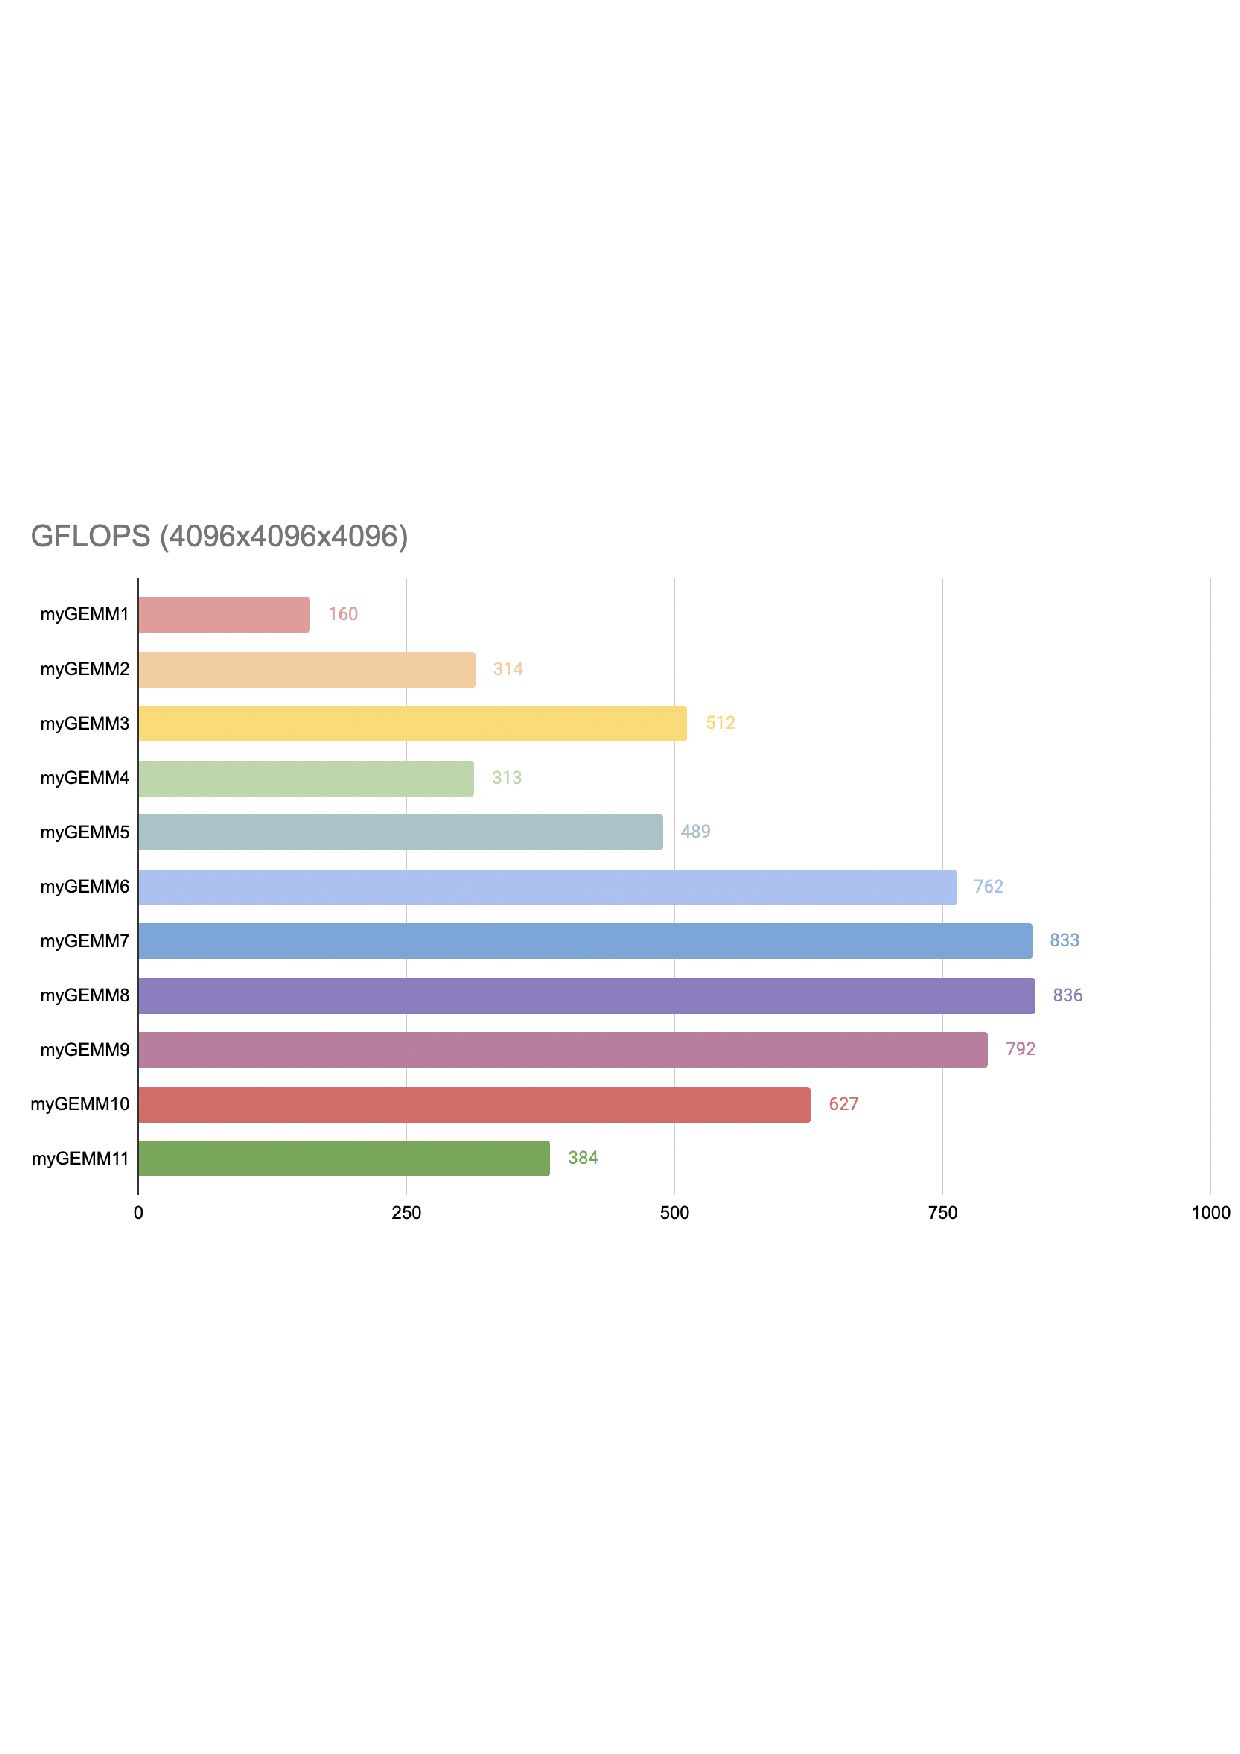
\includegraphics[width=\textwidth]{diagrams/kernel_4096.pdf}
        \\[-2cm] \centering \textbf{а)} Размер матрицы $4096 \times 4096$
    \end{minipage}
    \hfill
    \begin{minipage}[t]{0.45\textwidth}
        \centering
        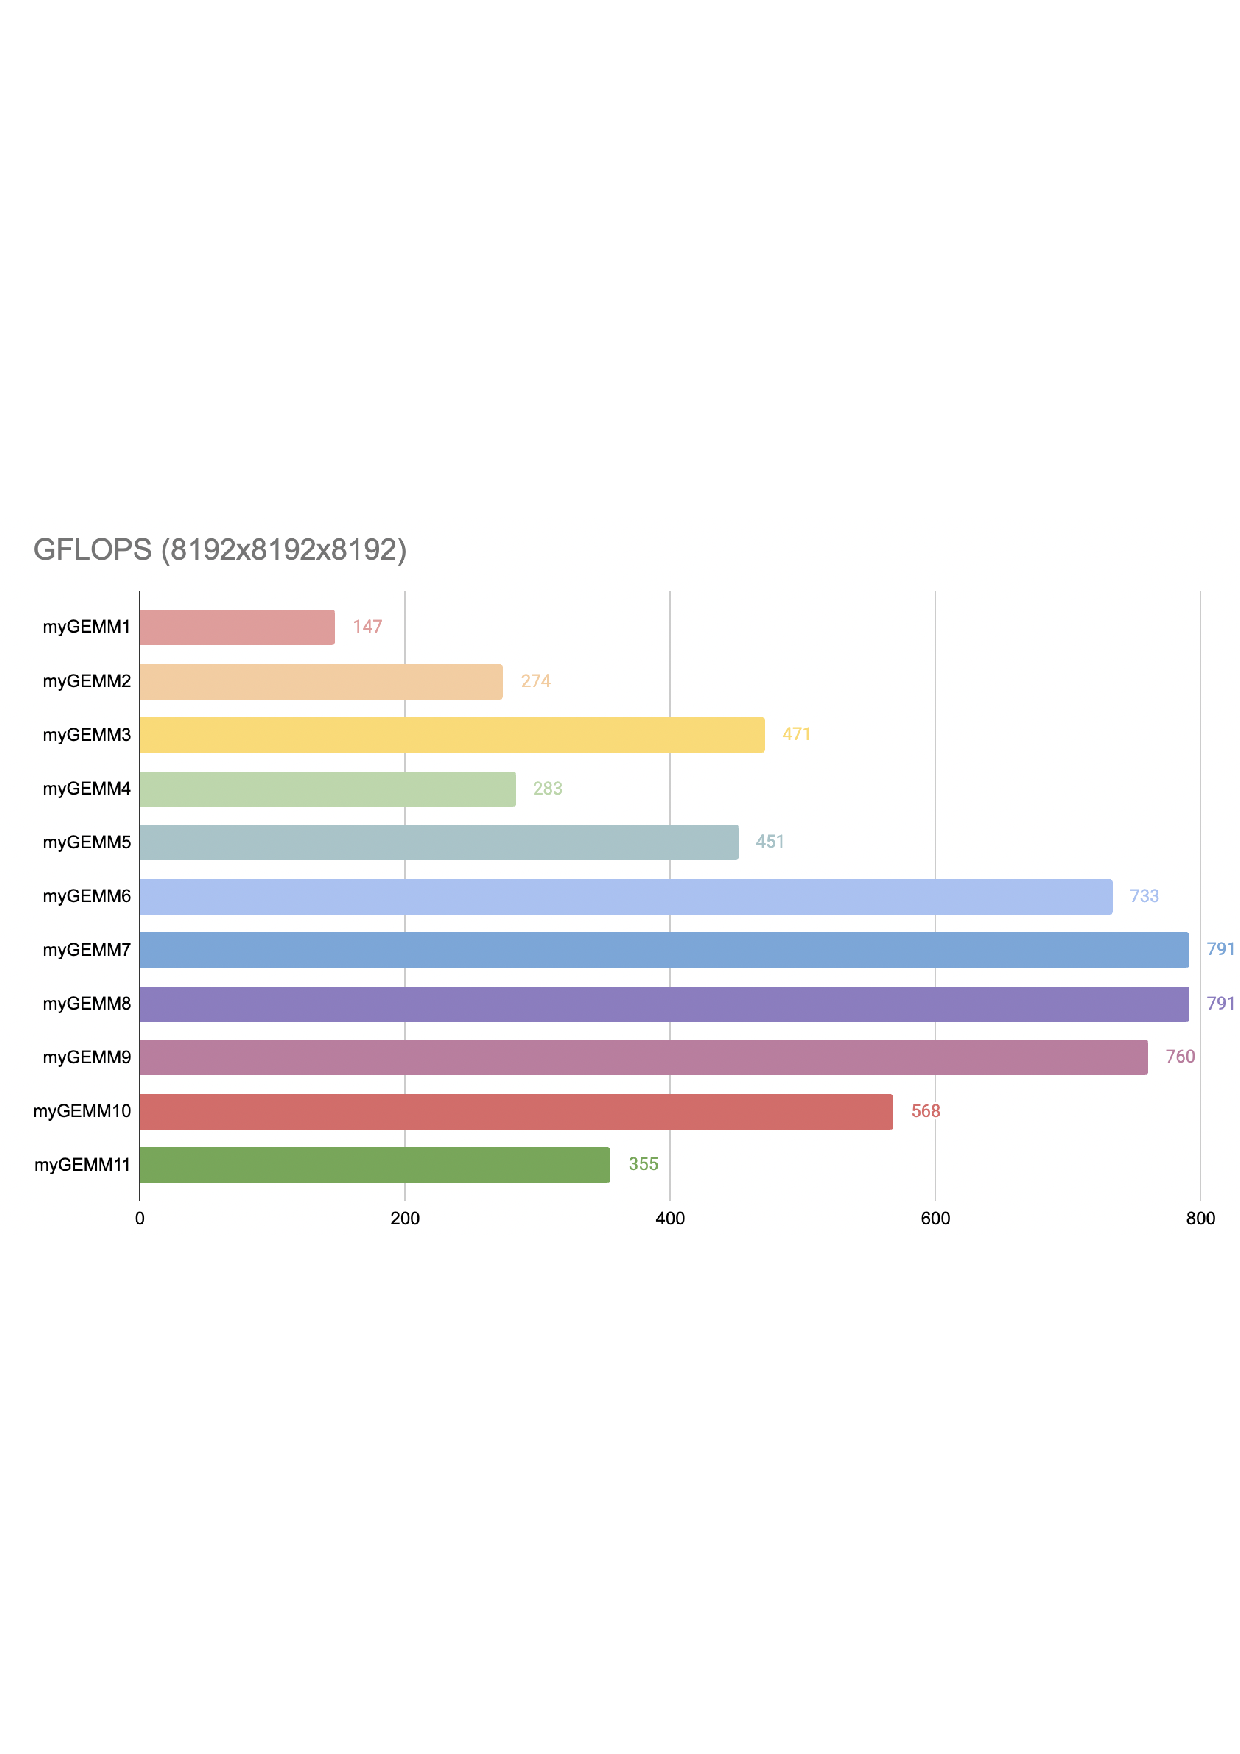
\includegraphics[width=\textwidth]{diagrams/kernel_8192.pdf}
        \\[-2cm] \centering \textbf{б)} Размер матрицы $8192 \times 8192$
    \end{minipage}
    \vspace{-1.5cm}
    \caption{Динамика производительности вычислительных ядер в зависимости от стратегии работы с памятью}
    \label{fig:kernel-diagrams}
\end{figure}

Численные значения средней производительности (GFLOPS) для матрицы \(4096 \times 4096\): Kernel~1 --- 160, Kernel~4 --- 313, Kernel~8 --- 836. Для матрицы \(8192 \times 8192\): Kernel~1 --- 147, Kernel~4 --- 283, Kernel~8 --- 791. Таким образом, комбинация двумерного блочного разбиения и регистровой оптимизации (\texttt{Kernel 8}) обеспечивает увеличение производительности в 5,2-5,7 раз в сравнении с базовой реализацией для двух масштабов матриц.

Детальный анализ показал, что итоговая производительность на UMA-архитектуре напрямую зависит от эффективности использования памяти:

\begin{itemize}
    \item \textbf{Базовое ядро (Kernel 1)} продемонстрировало наименьшую эффективность (около 120-160 GFLOPS) ввиду высокой конкуренции потоков за доступ к пропускной способности памяти;
    \item \textbf{Векторизация чтения (Kernel 4)} увеличила пропускную способность за счет использования типов \texttt{float4}, дав прирост производительности примерно в 2 раза в сравнении с базовой версией;
    \item \textbf{Комбинация двумерного блочного разбиения и регистровой оптимизации} (\texttt{Kernel 8}) позволила достичь максимальной производительности (более 750 GFLOPS). Загрузка блоков матриц в локальную память общего доступа и аккумуляция промежуточных сумм в регистрах минимизировали количество обращений к глобальной памяти.
\end{itemize}

Анализ результатов для ядер с близкими оптимизациями позволил выявить влияние конкретных методов на итоговую эффективность. Добавление регистровой оптимизации к двумерному тайлингу (сравнение \texttt{kernel 6} и \texttt{kernel 7}) обеспечивает прирост производительности примерно на 9\%.

Минимальный разброс значений для ядра kernel 8 (стандартное отклонение составляет 1-5 GFLOPS) подтверждает воспроизводимость результатов и стабильность условий проведения эксперимента.

\section{Заключение}

В ходе выполнения практики были решены поставленные задачи:
\begin{itemize}
    \item проведена серия замеров производительности различных ядер из проекта myGEMM на платформе macOS при трансляции через cl2Metal;
    \item определено влияние различных приёмов на эффективность вычислений графического процессора. Доказано, что комбинация двумерного тайлинга и регистровой оптимизации \texttt{kernel 8} обеспечивает прирост производительности в 5,2-5,7 раз относительно наивной реализации;
    \item разработан Python-комплекс для автоматизации сбора различных показателей. Устранено ограничение транслятора  \texttt{cl2Metal};
    \item проведена проверка стабильности результатов на основе 50 итераций для каждого вычислительного ядра.
\end{itemize}

Исходный код разработанного инструментария, конфигурационные файлы для CI/CD размещены в открытом доступе. Структура репозитория и описание конфигураций позволяют воспроизвести эксперименты на аналогичном аппаратном обеспечении.

Репозиторий проекта: \url{https://github.com/NewsPGG/myGEMM}.

\end{document}